\section{Introducci�n}

En el presente cap�tulo se establece el alcance del proyecto. Se plantean los objetivos tal y como fueron formulados originalmente y luego se los clasifica en las tres partes fundamentales del proyecto: \textit{investigaci�n}, \textit{implementaci�n} y \textit{aplicaci�n}. Estas son ponderadas en funci�n de la importancia que tienen en el mismo, y por consiguiente la importancia que se les dio. Luego, se resume la estructura de la aplicaci�n final, de manera de poder comprender a todo el proyecto en su conjunto. Finalmente se presenta un esquema del resto de la documentaci�n donde se explican los elementos necesarios para desarrollar cada parte de dicha aplicaci�n.
 
\section{Objetivos del proyecto}

El presente proyecto de fin de carrera tiene varios objetivos. En primer lugar se busca evaluar la capacidad de procesamiento de dispositivos m�viles para aplicaciones de procesamiento de im�genes y estudiar el desempe�o de diferentes algoritmos. Esto implica que se deben estudiar los diferentes dispositivos disponibles en el mercado. Por otro lado poder aplicar lo investigado para desarrollar una aplicaci�n de realidad aumentada completa funcionando sobre un dispositivo m�vil y en tiempo real. Finalmente se quiere utilizar dicha aplicaci�n para abordar un problema real, el \textit{recorrido interactivo con realidad aumentada} para museos.

Los objetivos anteriores pueden resumirse en las tres tareas fundamentales del proyecto, que se expresan a continuaci�n:

\begin{itemize}
\item[1.] \textbf{Investigaci�n:} Comprensi�n de la arquitectura de las plataformas m�viles y de sus plataformas de desarrollo, con el objetivo de implementar los distintos algoritmos y \textit{software} en general en las mismas. Estudio de las diferentes maneras de lograr la realidad aumentada, elecci�n de los algoritmos a utilizar y su comprensi�n, desarrollo de nuevos algoritmos y variantes de algoritmos existentes. Aprendizaje de herramientas en general.
\item[2.] \textbf{Implementaci�n}: Integraci�n de los distintos bloques para lograr la realidad aumentada. Implementaci�n de bloques l�gicos accesorios que faciliten la integraci�n de los primeros. Validaci�n de los algoritmos utilizados y desarrollados.
\item[3.] \textbf{Aplicaci�n}: Implementaci�n de una aplicaci�n completa en la que el usuario ingrese al museo, se ubique dentro de �l, se dirija a un cuadro, reciba informaci�n respecto del mismo y finalmente experimente la realidad aumentada sobre la obra.
\end{itemize}

Cada una de ellas se jerarquiz� en funci�n de la importancia que se les dio en el proyecto, as� como tambi�n el tiempo que se les dedic�:

$$
\begin{array}{|c|c|} \hline
\textbf{Frente de trabajo}			& \textbf{Porcentaje} \\ \hline
\small \textbf{Investigaci�n}		&	50\% \\ \hline
\small \textbf{Implementaci�n}	& 30\% \\ \hline
\small \textbf{Aplicaci�n}			& 20\%  \\ \hline
\end{array}
$$

Lo que la tabla anterior intenta reflejar es que el foco principal del proyecto es la investigaci�n, evaluaci�n de algoritmos y su migraci�n a plataformas m�viles. La aplicaci�n es un objetivo secundario que ayuda a validar los conceptos estudiados en las etapas de investigaci�n e implementaci�n. 

\section{Estado del arte}
Para llevar a cabo los objetivos planteados es bueno tener un contexto del estado del arte en cuanto al desarrollo de aplicaciones de realidad aumentada. Existen en la actualidad m\'ultiples kits de desarrollo comerciales para aplicaciones de realidad aumentada, en los que de manera sencilla, se logran este tipo de aplicaciones con desempe\~nos  muy buenos. Tal es el caso de \textit{Metaio} \cite{metaio12}, \textit{Vuforia} \cite{vuforia12}, \textit{String} \cite{string12} y \textit{Aurasma} \cite{aurasma12}. Por su parte, \textit{Layar} \cite{layar12}, es tambi\'en un kit de desarrollo para aplicaciones de realidad aumentada, pero se especializa en el agregado de contenido digital s\'olo sobre p�ginas impresas como revistas y cat�logos. Ninguna de las herramientas anteriores es gratuita y tampoco \textit{open source}. En la Figura \ref{fig: metaioystring} se muestra un ejemplo que incluye por defecto \textit{Metaio} y otro que incluye \textit{String}.

\begin{figure}[H]
\centering
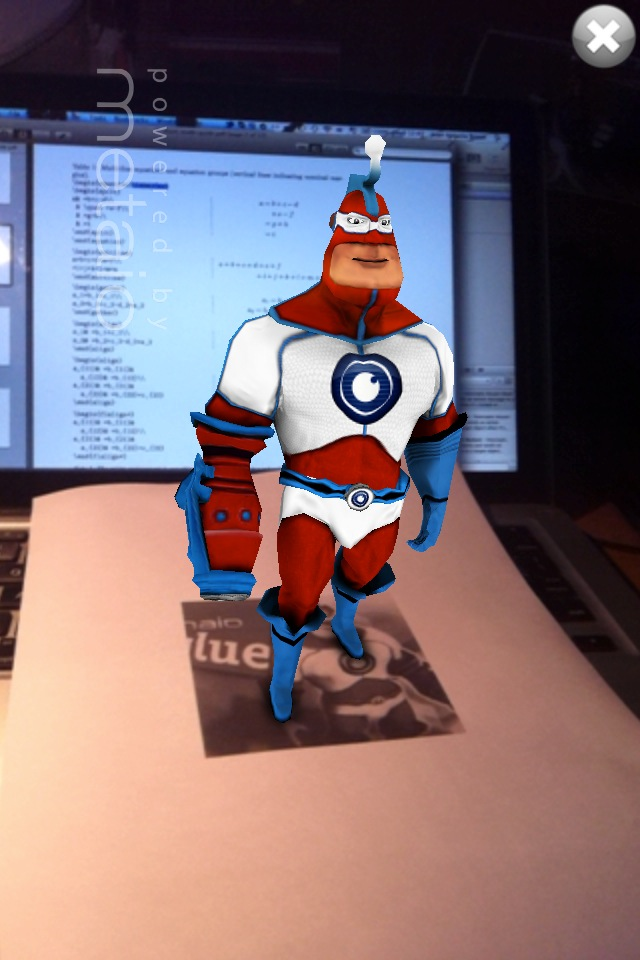
\includegraphics[scale=0.222]{figs_alcance/metaio.png}
\caption{Izq}
\label{fig: metaioystring}
\end{figure}

